\documentclass[a4paper, 12pt]{article}
\usepackage[T1]{fontenc}
\usepackage[utf8]{inputenc}
\usepackage[left=25mm,top=25mm,right=25mm,bottom=25mm]{geometry}
\usepackage{graphicx}
\usepackage[margin=0.5cm]{caption}

\usepackage{newtxtext,newtxmath}
\usepackage{tabularx}
\usepackage{blindtext}
\usepackage{tocloft}
\usepackage{indentfirst}
\usepackage{cancel}

\usepackage{tikz}
\usepackage{wrapfig}

\usepackage{pgfplots}

\tolerance=1
\emergencystretch=\maxdimen
\hyphenpenalty=10000
\hbadness=10000
\renewcommand{\contentsname}{İÇİNDEKİLER}
\renewcommand{\figurename}{Şekil}
\renewcommand\refname{KAYNAKLAR}
\renewcommand{\cfttoctitlefont}{\hspace{6.1cm}\large\bfseries\vspace{2cm}}
\renewcommand{\cftaftertoctitle}{\hfill}
\DeclareCaptionType{equ}[][]

\usepackage{xfrac}
\usepackage[unicode]{hyperref}
\hypersetup{
    colorlinks,
    citecolor=black,
    filecolor=black,
    linkcolor=black,
    urlcolor=black
}

\makeatletter
% argument #1: any options
\newenvironment{customlegend}[1][]{%
    \begingroup
    \let\addlegendimage=\pgfplots@addlegendimage
    \let\addlegendentry=\pgfplots@addlegendentry
    % inits/clears the lists (which might be populated from previous axes):
    \pgfplots@init@cleared@structures
    \pgfplotsset{#1}%
}{%
    % draws the legend:
    \pgfplots@createlegend
    \endgroup
}%
\makeatother



\begin{document}

\thispagestyle{empty}
\begin{center}


\textbf{KARADENİZ TEKNİK ÜNİVERSİTESİ \\ MÜHENDİSLİK FAKÜLTESİ \\ BİLGİSAYAR MÜHENDİSLİĞİ BÖLÜMÜ}

\vspace{1cm}

\includegraphics[]{ktu_logo.jpg}

\vspace*{2cm}

\textbf{EULER RENK VE HAREKET BÜYÜTME \\ YÖNTEMLERİYLE VİDEODAN NABIZ TESPİTİ}

\vspace*{\fill}

\textbf{BİTİRME TASARIM PROJESİ}

\vspace*{\fill}

\textbf{Mirza ATLI \\ Doğukan DİKMEN \\ Halil İbrahim BAŞKAYA}

\vspace*{\fill}

\textbf{2020-2021 BAHAR DÖNEMİ}



\newpage

\pagenumbering{Roman}
\thispagestyle{empty}
\centering
\textbf{KARADENİZ TEKNİK ÜNİVERSİTESİ \\ MÜHENDİSLİK FAKÜLTESİ \\ BİLGİSAYAR MÜHENDİSLİĞİ BÖLÜMÜ}

\vspace*{\fill}


\textbf{EULER RENK VE HAREKET BÜYÜTME \\ YÖNTEMLERİYLE VİDEODAN NABIZ TESPİTİ}

\vspace*{\fill}


\textbf{BİTİRME TASARIM PROJESİ}

\vspace*{\fill}


\textbf{Mirza ATLI \\ Doğukan DİKMEN \\ Halil İbrahim BAŞKAYA}

\vspace*{\fill}
\textbf{2020-2021 BAHAR DÖNEMİ}


\newpage

\phantomsection
\addcontentsline{toc}{section}{IEEE ETİK KURALLARI}


{\centering
\includegraphics[width=70pt]{ieee.png}
\hfill
\begin{minipage}[b]{.6\textwidth}
\centering
\textbf{\LARGE IEEE Etik Kuralları\\\vspace{0.2cm}\hspace{0.3cm}IEEE Code of Ethics
}\vspace{0.7cm}
\end{minipage}
\hfill
\includegraphics[width=70pt]{ieee.png}}
\vspace{1cm}
\end{center}

\small
Mesleğime karşı şahsi sorumluluğumu kabul ederek, hizmet ettiğim toplumlara ve üyelerine en yüksek etik ve mesleki davranışta bulunmaya söz verdiğimi ve aşağıdaki etik kurallarını kabul ettiğimi ifade ederim:
\begin{enumerate}
\itemsep0em 
\item Kamu güvenliği, sağlığı ve refahı ile uyumlu kararlar vermenin sorumluluğunu kabul etmek ve kamu veya çevreyi tehdit edebilecek faktörleri derhal açıklamak;
\item Mümkün olabilecek çıkar çatışması, ister gerçekten var olması isterse sadece algı olması, durumlarından kaçınmak. Çıkar çatışması olması durumunda, etkilenen taraflara durumu bildirmek;
\item Mevcut verilere dayalı tahminlerde ve fikir beyan etmelerde gerçekçi ve dürüst olmak;
\item Her türlü rüşveti reddetmek;
\item Mütenasip uygulamalarını ve muhtemel sonuçlarını gözeterek teknoloji anlayışını geliştirmek;
\item	Teknik yeterliliklerimizi sürdürmek ve geliştirmek, yeterli eğitim veya tecrübe olması veya işin zorluk sınırları ifade edilmesi durumunda ancak başkaları için teknolojik sorumlulukları üstlenmek;
\item	Teknik bir çalışma hakkında yansız bir eleştiri için uğraşmak, eleştiriyi kabul etmek ve eleştiriyi yapmak; hatları kabul etmek ve düzeltmek; diğer katkı sunanların emeklerini ifade etmek;
\item	Bütün kişilere adilane davranmak; ırk, din, cinsiyet, yaş, milliyet, cinsi tercih, cinsiyet kimliği, veya cinsiyet ifadesi üzerinden ayırımcılık yapma durumuna girişmemek;
\item	Yanlış veya kötü amaçlı eylemler sonucu kimsenin yaralanması, mülklerinin zarar görmesi, itibarlarının veya istihdamlarının zedelenmesi durumlarının oluşmasından kaçınmak;
\item	Meslektaşlara ve yardımcı personele mesleki gelişimlerinde yardımcı olmak ve onları desteklemek.

\end{enumerate}

\begin{flushright} IEEE Yönetim Kurulu tarafından Ağustos 1990’da onaylanmıştır.\end{flushright}

\normalsize
\newpage

\phantomsection
\addcontentsline{toc}{section}{ÖNSÖZ}

\hspace{5cm}
\begin{center}
\large \textbf{ÖNSÖZ}
\end{center}
\vspace{1cm}

Tez çalışmamızın planlanmasında, araştırılmasında, yürütülmesinde ve oluşumunda ilgi ve desteğini esirgemeyen, engin bilgi ve tecrübelerinden yararlandığımız, yönlendirme ve bilgilendirmeleriyle çalışmamızı bilimsel temeller ışığında şekillendiren sayın hocamız Prof. Dr. Cemal KÖSE'ye sonsuz teşekkürlerimizi sunarız.

\vspace{2cm}
\begin{flushright}
Mirza ATLI \\
Doğukan DİKMEN \\
Halil İbrahim BAŞKAYA \\ 
\vspace{0.2cm}

Trabzon 2020
\end{flushright}
 
\newpage
\tableofcontents

\phantomsection
\addcontentsline{toc}{section}{İÇİNDEKİLER}


\newpage

\phantomsection
\addcontentsline{toc}{section}{ÖZET}

\begin{center}
	\large \textbf{ÖZET}
\end{center}

Projenin amacı; çıplak gözle görülmesi mümkün olmayan hareket ve renk değişimlerini görülebilir hale getirmek ve elde edilen bu bilgiler doğrultusunda standart video girişinden nabız bilgisini elde etmektir. Projede standart video girişi mekansal ayrıştırılır, bant filtrelerinden geçirilir. Elde edilen frekans aralığındaki sinyaller istenilen oranda çoğaltılarak ve sağlanan video girişi ile mekansal birleştirilerek, bahsedilen hareket ve renk değişimleri görünür hale getirilir.

Bu çalışma, temas yolu ile nabız ölçümü sakıncalı olan bireyler ve nörovasküler fonksiyonları, travma veya bir rahatsızlık sonucu bozulmuş bireyler gözetilerek geliştirilmiştir.  

\newpage
\pagenumbering{arabic}

\section{GENEL BİLGİLER}

\subsection{Giriş}
\begin{figure}[h]
        \centering
	    \setlength\tabcolsep{-2pt} % default value: 6pt
        \begin{tabular}{cccc}

	\includegraphics[width=3cm]{orj/orj1.jpg}	& \includegraphics[width=3cm]{orj/orj2.jpg} & \includegraphics[width=3cm]{orj/orj3.jpg} & \includegraphics[width=3cm]{orj/orj4.jpg}	 \\
	
		\includegraphics[width=3cm]{artt/artt1.jpg}	& \includegraphics[width=3cm]{artt/artt2.jpg} & \includegraphics[width=3cm]{artt/artt3.jpg} & \includegraphics[width=3cm]{artt/artt4.jpg}	 \\
        \end{tabular}

        \caption*{ Şekil 1: Üst sıra video girişi, alt sıra ise video çıkışıdır.}
        \label{tbl:giris-cikis}
\end{figure}


	
	İnsan derisininin kan dolaşımı ile renk değiştirdiğini, çıplak gözle görülmesi mümkün olmasa da bu değişimin görüntü işleme algoritmalarıyla ortaya çıkarılabileceği, öncesinde sayısal sonrasında ise görsel olarak sonuç üretilebileceği yapılan çalışmalar ile kanıtlanmıştır.\cite{poh2010non} Şekil \ref{tbl:giris-cikis}'da programın örnek giriş ve çıkışı gösterilmiştir. 

Bu projede Gauss ve Laplace piramitlerinin, bahsi geçen gözle görülmesi zor değişimlerin ortaya çıkarılmasında nasıl kullanılacağına değinilecektir. Kullanıcıdan alınan video zamansal ve mekansal olarak ayrıştırılacak, beklenilen frekans aralığındaki frekanslar güçlendirilecek, dışında kalan frekanslar güçsüzleştirilecek ve video tekrar bir araya getirilecektir. Sinyal üzerinde, belirli bir frekans aralığının güçlendirilmesi işlemlerinde oynadıkları role matematiksel ispat ile değinilecek ve uygulanması gereken her adım, görsel örnekler ile desteklenecektir. 


Nabız takibi bir çok hastalıkta önemli olduğundan, temassız nabız takibi yapılabilmesi de önemlidir. Temassız nabız ölçümü gerektiren durumlara; entübe bebekler, yüksek ölçüde yanıklara sahip hastalar ve plastik alerjisi olan bireyler örnek gösterilebilir. Projede kullanılan yöntem ile bebeklerin nefes alışverişlerinin takibi de kolaylaştırılabilir. Diyabet veya travmaya bağlı gelişen, sempatik sinir sisteminde hasar meydana gelmiş hastaların cilt düzeyinde asimetrik kan dağılımı da proje sayesinde gözlemlenebilir. 




\subsection{Video Giriş/Çıkış Standartları}

Matematiksel ispata ve algoritmanın gerçekleştirilmesine geçmeden önce projenin kabul edilebilir çalışma şartlarından bahsedilmesi gerekir. Kullanıcıdan alınan videonun çekim anında, oynatma anındaki FPS ile çekim yaptığı varsayılır ve işlem adımları buna göre uygulanır. Standart dışı veri sıkıştırma algoritmalarının kullanılmaması önerilir fakat proje, standart olarak kabul edilmiş algoritmalar ile sorunsuz çalışmaktadır. Girişin dikey ve yatay boyutları aynı olup 2'nin katları olması, Gauss piramitlerinin oluşturulmasında yaşanacak olan kalite kaybını az da olsa azaltmaktadır. Bu azalma, kullanıcıdan alınan videonun kenarlarında bulunan işlemler açısından gereksiz bölgelerinin kırpılması ile önem kazanmaktadır zira sağlanan videoların büyük çoğunluğunda ilgi odağı bölge merkezdedir ve genellikle geri kalan yerler ile ilgilenilmemektedir. 

İdeal olarak video girişinin; 30 FPS'in üstündeki değerlerde çekim yapılmış olması, ilgi odağının merkezde bulunuyor olması ve görüntünün çoğunu kaplıyor olması, çekim FPS'i ve ilgilenilen frekans aralığına göre değişkenlik gösterse de 10 saniyeden kısa olmaması ve gerçek zamanlı işlem yapılabilmesi için video çözünürlüğü ve piramit seviye sayısının önemli ölçüde fark yaratmayacak kadar arttırılmaması gereklidir. Çalışmamız sonucunda, bahsedilen ideal koşulları sağlamayan videolarda da kabul edilebilir sonuçlar göstermiştir. 

Video süresi, işlem zamanını üssel değil lineer olarak arttırır, bundan ötürü zamandan ziyade video boyutuna dikkat edilmelidir. Programın çıktısı olarak giriş videosu -veya video kamerasından alınan canlı yayın- ile aynı FPS değerinde, değişimin arttırıldığı bir video üretilir ve kullanıcıya gerçek zamanlı olarak gösterilir. Girişten farklı olarak, çıkıştaki videonun sıkıştırılmasında herhangi bir sakınca yoktur.

Dikkat edilmesi gereken bütün kısıtlara, ayrıntılı olarak Bölüm \ref{sec:kisitlar}'te değinilmiştir. 
 


\newpage


\section{MATEMATİKSEL İZAH}
Bu kısımda zamansal işlemlerin, videodaki değişimleri nasıl büyüteceği birinci dereceden Taylor serileri ile açıklanacaktır. Burada yapılan işlemler anlatım kolaylığı olması açısından tek boyutlu uzay üzerinde uygulanmıştır. Aynı işlemlerin 2 boyutlu uzaydaki işlem adımları aynıdır. 

\subsection{Birinci Dereceden Hareket}{\label{birinci-dereceden}}
$x$ pozisyonundaki, $t$ zamanındaki pikselin parlaklığını $I(x,t)$ fonksiyonu ile ifade edelim. Projede istenen hareketlerin bulunması gerektiğinden öteleme hareketlerinin de bulunması gerekmektedir. Bahsi geçen yöntem ile büyütme, faz değiştirme gibi değişim olayları saptanamaz. Gözlemlenen piksel parlaklığı değişimini $\delta(t)$ ile ifade edelim. Birleştirirsek; 

\begin{equation}
\label{eqn:bir}
G(x,t) = f(x+\delta(t)) 
\end{equation}

Başlangıçta değişim $\delta(0)=0$ olduğundan Denklem \ref{eqn:bir}'de $I(x,0) = f(x)$ değerini alır. Bu değerin yaratabileceği sorunlara Bölüm \ref{sec:birlestirme}'te değinilecektir.

Denklem \ref{eqn:bir}'te $\delta(t)$ fonksiyonu $0$ ile çarpılırsa statik bir girişte verilen sinyalin değişimi ne olursa olsun çıkışta değişmeyen bir sinyal gözlemlenir. Projede istenen, değişimin daha gözle görülebilir hale getirilmesi gerektiğinden $\delta(t)$ fonksiyonunun 1'den büyük bir katsayı ile çarpılması durumunda istenen sonuç elde edilmiş olur. Yani;

\begin{equation}
\label{eqn:iki}
	\text{\textit{Ç}}(x,t) = f(x+\alpha \cdot \delta(t)), \quad \alpha > 1 
\end{equation}

İstenen değişim, $\delta(t)$'nin , birinci dereceden Taylor serisi ile de ifade edilebilir. $t=0$ anında $\delta(0)=0$ olacağından Taylor serisinde başlangıç anındaki $\delta(t)$'yi yazmamıza gerek yoktur. $t$ anındaki, $x$ konumundaki pikselin parlaklığını ifade eden, herhangi bir katsayı ile çarpılmamış fonksiyonun birinci dereceden Taylor açılımı;

\begin{equation}
\label{eqn:uc}
	G(x,t) \approx f(x) + \delta(t) \cdot\frac{\partial f(x)}{\partial x}
\end{equation}

Denklem \ref{eqn:uc}'de belirtilen $\delta(t)$ ve ilgili türev kısmının değişimdeki artışı ifade ettiği, $f(x)$'in de genel anlamda değişimi ifade ettiği anlaşılmaktadır. Bu değişimdeki artışın, projede istenen aralığın içinde kalması ve geriye kalan kısımların artırılmaması için bant geçiren süzgeçten geçirilmesi gerekmektedir. Uygulanan bu süzgeçlerin, çıkışta ani değişimlere yol açmaması için \textit{butterworth} süzgecinden geçirilmesi de gerekmektedir.

Bahsi geçen süzgeçlerden geçirilen sinyalin, daha önceden belirtilen $\alpha$ katsayısı ile çarpılması durumunda sinyalin istenilen aralıktaki değişimi gözlemlenmiş olur. Bu sonucu, en başta sağlanan sinyal ile toplanması durumunda istenilen değişimin \textit{abartılarak} sonuca aktarılması gözlemlenir. Yani; 

\begin{equation}
\label{eqn:dort}
	 \text{\textit{Ç}}(x,t) \approx G(x) + \alpha \cdot \delta(t) \cdot\frac{\partial f(x)}{\partial x}\;, \quad \alpha > 1
\end{equation}


Şekil \ref{sekil:bir}'de görülebileceği gibi $I(x,t)$ fonksiyonunda genellikle sabit kalan bir $f(x)$(\ref{graf1:fx}) ve zamana göre değişime uğrayan bir $\delta(t)$ fonksiyonu mevcuttur. Şekildeki $I(x,t)$ fonksiyonuna etki eden birden fazla \textit{girişim} fonksiyonu olmadığı için önceden bahsedilen süzgeçlerden geçirilmeye ihtiyaç duyulmamıştır. $\delta(t)$ fonksiyonu ayrıştırılıp, 1'den büyük bir katsayı ile çarpıldığında $\text{\textit{Ç}}(x,t)$(\ref{graf1:fx+dd}) elde edilmiş olur.

\begin{wrapfigure}{r}{0.45\textwidth}
	\centering
	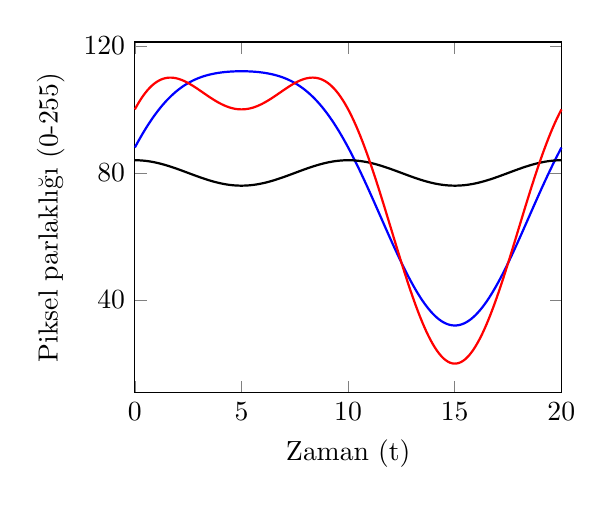
\begin{tikzpicture}
    \begin{axis}[
     width=7cm,
     clip=false,
     xlabel=Zaman (t),
     ylabel=Piksel parlaklığı (0-255),
     xmin=0,xmax=2*pi,
     %axis lines=left,
     %axis x line=middle,
     %axis y line=left,
     xtick={0,1.57,3.14,4.71,6.28},
     xticklabels={$0$, $5$,$10$,$15$,$20$},
	    yticklabels={$0$, $40$, $80$, $120$, $160$, $200$, $240$}
     ]

	    \addplot[domain=0:2*pi,samples=200,blue, thick]{sin(deg(x)) + 1/5 * cos(2*deg(x))};\label{graf1:fx}
	    \addplot[domain=0:2*pi,samples=200,black, thick]{ 1/10 * cos(deg(2*x))};\label{graf1:fx+d}
	    \addplot[domain=0:2*pi,samples=200,red, thick]{ sin(deg(x)) + 1/2 * cos(2*deg(x)) };\label{graf1:fx+dd}
    \end{axis}


\end{tikzpicture}
	\caption{$f(x) + \delta(t)$ (\ref{graf1:fx}),\quad $\delta(t)$ (\ref{graf1:fx+d}),\quad \newline $ f(x) + \alpha \cdot \delta(t) $ (\ref{graf1:fx+dd}) şeklinde eğrilerle belirtilmiştir. $f(x)$, güçlü bir sinüs dalgası ile güçsüz ve frekansı daha yüksek bir kosinüs dalgasının toplamıdır. Bu güçsüz dalga $\delta(t)$'dir ve $\alpha$ ile çarpılırsa kırmızı ile belirtilen, değişimin abartıldığı bir eğri çizilmiş olur.}
\label{sekil:bir}
	\vspace{-1cm}
\end{wrapfigure}



Şekil \ref{sekil:bir}'deki girişim fonksiyonu ve bu fonksiyonun Taylor serisi ile yakınsaması çok yakın olduklarından aradaki farkı gözlemlemek zordur. Taylor serisi ile girişim yaratan frekansların yakınsamasının alınması ile bahsedilen süzgeçler ile gereksiz frekanslar ayrıştırılır ve yakınsama işlemi uygulanır. İstenilen aralıktaki frekanslarda, Bölüm \ref{mat-kisitlar}'te bahsedilen artan $\alpha$ değerinin yaratacağı sorunları ortadan kaldırmak için, artan frekanslarda \textit{butterworth} filtresi uygulanacaktır. Bu proje kapsamında ortalama insan nabız aralığı filtreleneceğinden $0.7\:Hz$ ile $2.0\:Hz$ aralığı kullanılacaktır. Ortalama bebek nabzı yaşa ve diğer faktörlere (uyku, stres hali vb.) göre büyük değişiklikler gösterse de ortalama olarak $1.6\:Hz$ ile $2.05\:Hz$ arasında seçilebilir.  

\subsection{Kısıtlar}{\label{mat-kisitlar}}

Önceki bölümde bahsedilen Taylor serisi ile yakınsama yönteminin yetersiz kaldığı duruma örnek olarak $\delta(t)$'nin frekansı ve genliği yüksek olduğu durum verilebilir. Genliği ve frekansı hali hazırda yüksek olan bu sinyalin $\alpha$ katsayısı ile çarpılması istenmeyen kalıntılarının çıkışa aktarılmasını sağlar ve bu istenmeyen bir durumdur. Düşünülenin aksine $\alpha$ değerinin sabit, $\delta(t)$ sinyalinin değişken frekans ve genliğinin olması durumunda farklı sinyal güçlendirme sonuçları oluşmaktadır. Aynı $\alpha$ değeri için aynı sonuç beklenemeyeceğinden, çıkış olarak bireyin nabız görüntüsü verildiğinde düşük nabızlarda şiddetli renk değişimi gözlemlenirken yüksek nabıza sahip bireylerdeki renk değişimi şiddetsiz gözlemlenebilir. Kabul ettiğimiz üst değer $2.0\:Hz$ ile $0.7\:Hz$ arasındaki frekans farkı göreli olarak fazla olduğundan $\alpha$ değeri dikkatle seçilmelidir. 

Dikkatle seçilmesi, önceden de bahsedildiği gibi ilgilenilen frekans aralığı daraldıkça $\alpha$ katsayısının arttırılmasını gerektirir. Alttaki görselde de görülebileceği üzere sadece ilgili frekans aralığının darlığı değil, ilgilenilen aralığın göreli olarak yüksek frekanslı olması durumunda $\alpha$'nın normalde seçilmesi gerekenden daha düşük bir değerde seçilmesi gerekmektedir.


\begin{figure}[ht]
	\centering
\begin{tabular}{cc}
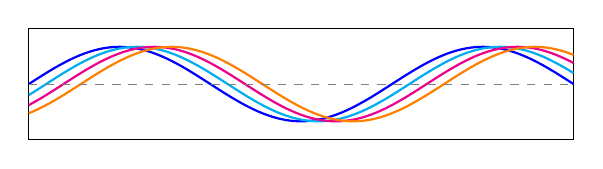
\begin{tikzpicture}
    \begin{axis}[
     clip=false,
	    height=3cm, width=8.5cm,
	    xmin=0,xmax=2*pi,
	    ytick=\empty,
	    ymin=-1.5,
	    ymax=1.5,
	    xtick=\empty,
     ]
	    \addplot[domain=0:2*pi,samples=200,blue, thick]{sin(deg(1.5*x))};\label{orj-sinyal}
	    \addplot[domain=0:2*pi,samples=200,cyan, thick]{sin(deg(1.5*x - 0.3))};\label{sinyal2}
	    \addplot[domain=0:2*pi,samples=200,magenta, thick]{sin(deg(1.5*x - 0.6))};\label{sinyal3}
	    \addplot[domain=0:2*pi,samples=200,orange, thick]{sin(deg(1.5*x - 0.9))};\label{sinyal4}
	    \addplot[domain=0:2*pi, dashed, gray]{0*x};

    \end{axis}
\end{tikzpicture}

&
\hspace*{0.3 cm}

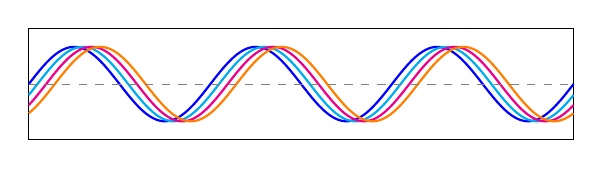
\begin{tikzpicture}
    \begin{axis}[
	    clip=false,
	    height=3cm, width=8.5cm,
		    ymin=-1.5,
	    ymax=1.5,    xmin=0,xmax=2*pi,
    	    ytick=\empty,
	    xtick=\empty,
 ]
	    \addplot[domain=0:2*pi,samples=200,blue, thick]{sin(deg(3*x))};
	    \addplot[domain=0:2*pi,samples=200,cyan, thick]{sin(deg(3*x - 0.3))};
	    \addplot[domain=0:2*pi,samples=200,magenta, thick]{sin(deg(3*x - 0.6))};
	    \addplot[domain=0:2*pi,samples=200,orange, thick]{sin(deg(3*x - 0.9))};
	    \addplot[domain=0:2*pi, dashed, gray]{0*x};
    \end{axis}
\end{tikzpicture}

\vspace{0.3cm}
\\

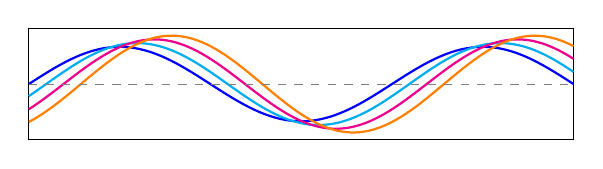
\begin{tikzpicture}
    \begin{axis}[
     clip=false,	    ymin=-1.5,
	    ymax=1.5,
	    height=3cm, width=8.5cm,
	    xmin=0,xmax=2*pi,
	    ytick=\empty,
	    xtick=\empty,
     ]
	    \addplot[domain=0:2*pi,samples=200,blue, thick]{sin(deg(1.5*x))};
	    \addplot[domain=0:2*pi,samples=200,cyan, thick]{1.1*sin(deg(1.5*x - 0.3))};
	    \addplot[domain=0:2*pi,samples=200,magenta, thick]{1.2*sin(deg(1.5*x - 0.6))};
	    \addplot[domain=0:2*pi,samples=200,orange, thick]{1.3*sin(deg(1.5*x - 0.9))};
	    \addplot[domain=0:2*pi, dashed, gray]{0*x};
    \end{axis}
\end{tikzpicture}
	
&

\hspace{0.3cm}
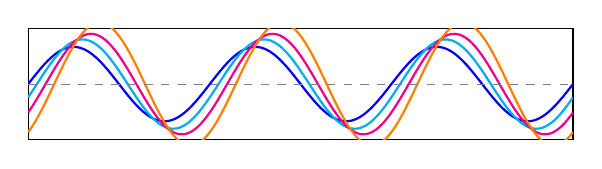
\begin{tikzpicture}
    \begin{axis}[
     clip=true,	    ymin=-1.5,
	    ymax=1.5,
	    height=3cm, width=8.5cm,
	    xmin=0,xmax=2*pi,
	    ytick=\empty,
	    xtick=\empty,
     ]
	    \addplot[domain=0:2*pi,samples=200,blue, thick]{sin(deg(3*x))};
	    \addplot[domain=0:2*pi,samples=200,cyan, thick]{1.2*sin(deg(3*x - 0.3))};
	    \addplot[domain=0:2*pi,samples=200,magenta, thick]{1.35*sin(deg(3*x - 0.6))};
	    \addplot[domain=0:2*pi,samples=200,orange, thick]{1.65*sin(deg(3*x - 0.9))};
	    \addplot[domain=0:2*pi, dashed, gray]{0*x};
    \end{axis}
\end{tikzpicture}
	


\end{tabular}
\caption{$Y$ ekseni parlaklığı, $X$ ekseni ise konumu ifade etmektedir. Üst sıra ideal sinyal güçlendirmenin, alt sıra ise proje kapsamındaki yönteminin sonuçlarınının temsilidir. Orijinal sinyal(\ref{orj-sinyal}), artan $\alpha$ katsayısı ile çarpılarak güçlendirilmiş sinyaller(\ref{sinyal2}, \ref{sinyal3}, \ref{sinyal4}) bulunur. Artan frekans ve $\alpha$ katsayısı ile ideal güçlendirmeden sapmalar gözlemlenir. }
\end{figure}

\newpage
\section{PROJE TASARIMI}


Proje kapsamında kullanıcıdan alınan video sekansından nabız bilgisi görsel olarak sunulacak şekilde tasarlandı. Projenin çekirdek kodu, tasarım ve test etme kolaylığı açısından Python ile prototimi geliştirildi. Performans gözetilerek C++'da yeniden yazıldı. Fourier dönüşümünden elde edilen bilgilerin görsel sunumu ve tezde kullanılacak görsellerin oluşturulması için Python'dan yararlanıldı. Kullanıcıdan bilgi almak ve program çıktılarını toplu bir şekilde tek bir yerde görüntülemek için C++/C\# kullanıldı.

Beklenen çıktının gözlemlenebilmesi için Bölüm \ref{mat-kisitlar}'de de değinilen değerlerin değiştirilebilmesi için C\# ile oluşturulan arayüz kullanılacaktır. 

\vspace{-0.55cm}

\begin{figure}[h]
\centering
\makebox[\linewidth]{
  \setlength\fboxsep{0cm}%<- optional for padding
	\includegraphics[width=19cm]{UML.png}}	
	
	\caption{Proje adımlarının görsel gösterimi. Veri girişi[\ref{veri-girisi}], videodan Gauss piramitlerinin üretilmesi[\ref{gauss-piramit}], band geçiren süzgeçlerin uygulanması[\ref{band-geciren-suzgec}], Gauss piramitlerinden video üretilmesi[\ref{gauss-piramit-video}] ve orijinal video ile birleştirilmesi.  }
	\label{proje-tasarim-plan}
\end{figure}



Şekil \ref{proje-tasarim-plan}'de proje planının çalışma adımları gösterilmiştir. Ana başlık altında yapılması gereken hesaplamalar ve bu hesaplamalara adım adım örnekler verilerek aşağıdaki bölümlerde ilgili konulara değinilecektir.



\subsection{Veri Girişi}{\label{veri-girisi}}

Diğer implemantasyonların YQIF renk uzayında işlem yapmasına\cite{YQIF}  karşın bu projede geliştirilmiş olan yazılım, RGB renk uzayında işlem yapmaktadır. YQIF renk uzayında işlem yapılmasının, RGB renk uzayında işlem yapılmasına göre herhangi bir performans veya görsel üstünlük saptanamamıştır. Görselleştirme ve anlaşılma kolaylığı nedeniyle RGB uzayında işlem yapılmasına karar verilmiştir. 

Önceki tasarım ve prototipimizin aksine kırpma işlemine başvurulmamış, görüntü sekansının tamamını belleğe alınmadan görseller üzerinde işlem yapılmaya karar verilmiştir. Bu karar ile bellek kullanımını önemli ölçüde azaltırken piramit seviyesindeki artışın performansı düşürmesini önemli ölçüde azaltmıştır. 


\subsection{Görüntü Piramitlerinin Oluşturulması}
Görüntü işleme alanında, yüz ve nesne algılama gibi işlemlerde görüntünün yeniden boyutlandırılması veya boyutunun küçültülmüş hallerinin referans olarak kullanılması\cite{eulerian-piramit}\cite{eulerian-piramit-2}\cite{eulerian-piramit-3}  için alt örneklemesi gerekir. Bu durumlarda aynı görüntünün farklı çözünürlükteki halleri üzerlerinde işlem yapılmak üzere bellekte saklanır. Aynı görüntünün çözünürlüklerine göre sıralanması halinde, Şekil \ref{piramit-ornek}'te görülebileceği üzere \textit{görüntü piramidi} elde edilmiş olur. 

Görüntü piramitlerinin arasında sıkça kullanılan iki ana tür vardır. Bunlar \textit{Gauss Piramitleri} ve \textit{Laplace Piramitleri}dir. Laplace piramitleri, Gauss piramitlerinden elde edildiğinden ve proje kapsamında hareketin ortaya çıkardığı renk değişimini azaltmasında kullanılacağından önemlidir.


Belirtmekte fayda var; proje kapsamında görüntüdeki renk değişimi incelendiği için ana işlemler Gauss piramitleri ile gerçekleştirilecektir. Önceki çalışmaların aksine hem Gauss hem de Laplace piramitlerini kullanarak hareketin yol açtığı renk değişimini minimize ederek renk değişimi (proje kapsamında nabız bilgisini) elde edilecektir. Bu durumda işlem maliyeti artacak fakat elde edilen sonuçların kalitesinde de gözle görülür bir artışa neden olacaktır. Nabız algılama konusunda sadece Laplace piramitleri ile kanın kafanın içerisinde hareket ederken gözle fark edilemeyecek kadar küçük hareketlere yol açmasından faydalanarak nabız algılayabilen sistemler geliştirilmiştir\cite{YQIF}. Bu sistemlerde bireyin yüzünü göstermeyecek şekilde dönmüş olması veya maske takması nabız algılanmasında sakınca teşkil etmemektedir.

\subsubsection{Gauss Piramitleri}{\label{gauss-piramit}}

\begin{figure}[h]
	\centering
	\includegraphics[scale=0.25]{euler.jpg}
		\caption{Butterworth filtresi uygulanmış 4 seviyeli Gauss piramidi. }
	\label{ornek-gauss-piramit}
\end{figure}
\vspace{-0.5cm}



Gauss piramitlerinde, görüntü alt örnekleme yapılmadan önce 5x5 büyüklüğünde bir filtre uygulanır. Bu filtreye \textit{Gauss filtresi} denir. Piramit oluşturmak için indirgeme, piramitin üst basamaklarından tekrar ana görüntünün çözünürlüğüne erişmek için genişletme adımlarına ihtiyaç vardır. İndirgeme işleminde Denklem \ref{reduce-denklem}'te verilen bağıntıya göre işlemler uygulanır. Belirtmekte fayda var; Şekil \ref{ornek-gauss-piramit}'te gözlemlenen piramit basamaklarına Butterworth filtresi uygulanmıştır, bu bölümde bahsedilen piramit oluşturma işlemlerinden direkt olarak görseldeki sonuç gözlemlenmez.  


\begin{equation}{\label{reduce-denklem}}
	G_l(i,j) = \sum_{m=-2}^{2} \sum_{n=-2}^{2}w(m,n)\cdot G_{l-1}(2i+m, 2j+n)
\end{equation}

Denklem \ref{reduce-denklem}'da $l$ ile belirtilen, Şekil \ref{piramit-ornek}'te gösterilen seviyelerden herhangi biridir. Numaralandırma işlemi en alt, orijinal görüntüye $0$ vererek başlanır ve kademeler arttıkça seviye numarası da arttırılır. Aynı denklemde $w(m,n)$ ile belirtilen kısım ise uygulanması gereken 5x5 büyüklüğündeki Gauss filtresidir. 


Bahsedilen indirgeme işleminin konvolüsyondan farkı, konvolüsyondaki adım büyüklüğünün (işlem yapılacak pikseller arasındaki mesafenin) değeri 1 iken indirgeme işleminde bu adım büyüklüğü değeri 2'dir. Bu adım büyüklüğünden ötürü Gauss filtresi uygulandığında görüntünün çözünürlüğü yarı yarıya düşer. Projenin gerçekleştirilme aşamasında işlem zamanından tasarruf etmek adına piramidin ara seviyelerinin atlanarak sağlanan görüntüden istenilen piramit seviyesinin hesaplanması denenmiş fakat başarılı sonuçlar alınamamıştır. Bu durum, çözünürlüğü yüksek videolar için yüksek seviyeli piramitlerin oluşturulmasında fazla bellek kullanılmasına neden olmaktadır. 


Oluşturulan piramitin alt basamağından üst basamaklara çıkmak, yani genişletme işlemi yapmak için Denklem \ref{expand-denklem}'da verilen bağıntıya göre işlemler uygulanır. 



\begin{equation}{\label{expand-denklem}}
	G_{l,n}(i,j) = \sum_{p=-2}^{2} \sum_{q=-2}^{2}w(p,q)\cdot G_{l,n-1} \left( \frac{i-p}{2},\; \frac{j-q}{2} \right)
\end{equation}


Denklem \ref{expand-denklem}'te belirtilen $l$, Denklem \ref{reduce-denklem}'teki gibi seviyeyi, $w(p,q)$ de uygulanacak olan Gauss filtresini belirtmekedir. Denklem \ref{reduce-denklem} ile Denklem \ref{expand-denklem} arasındaki ilişkiyi anlayabilmek için Denklem \ref{expand-denklem} tek boyutta yazılırsa,



\begin{equation}{\label{reduce-ornek-bir}}
	\begin{gathered}	
	G_{l,n}(i) = \sum_{p=-2}^{2}\hat{w}(p) \cdot G_{l,n-1}\left(\frac{i-p}{2}\right) 
	\\
		\\
		G_{l,n}(4) = \hat{w}(-2)G_{l,n-1}\left(\frac{4+2}{2}\right) + 
		\cancel{ \hat{w}(-1)G_{l,n-1}\left(\frac{4+1}{2}\right) } + 
		\\
		\hat{w}(0)G_{l,n-1}\left(\frac{4}{2}\right) + 
		\cancel{\hat{w}(1)G_{l,n-1}\left(\frac{4-1}{2}\right) } + 
		\hat{w}(2)G_{l,n-1}\left(\frac{4-2}{2}\right)
	\end{gathered}
\end{equation}
\\

\begin{equation}{\label{reduce-ornek-iki}}
	G_{l,n}(4) = \hat{w}(-2)G_{l,n-1}(3) + \hat{w}(0)G_{l,n-1}(2) + \hat{w}(2)G_{l,n-1}(1)
\end{equation}

Denklem \ref{reduce-ornek-bir}'de $G$ fonksiyonunun girişi $i$ ve $j$ koordinatları, tam sayı haricinde bir değer alamayacağından denklemde tamsayı içermeyen kısımlar silinmiştir.
Proje kapsamında, bir görüntü sekansından elde edilen piramidin seviyeleri arasında değişkenlik gösteren detayları aramak yerine video içeriğinde değişkenlik gösteren kısımlar arandığı için; piramidin seviyeleri arasında değil, art arda gelen resim karelerinin oluşturduğu piramidin seviyeleri arasında fark aranacaktır.

%Şekil (\ref{ornek-gauss-piramit})'te beklenen piramit seviyeleri elde edilmiştir. 



\subsubsection{Laplace Piramitleri}{\label{laplace-piramit}}

\begin{figure}[h]
	\begin{center}
	\includegraphics[scale=0.25]{laplace.jpg}
	\caption{Butterworth filtresi uygulanmış 4 seviyeli Laplace piramidi.}
		\label{laplace-piramit-ornek}
	\end{center}
\end{figure}
\vspace{-0.5cm}

Laplace piramitlerinin Gauss piramitlerinden elde edileceğinden bahsetmiştik. Laplace piramitlerinin basamaklarının elde edilebilmesi için Gauss piramidinin oluşturulması gerekmektedir. Laplace piramidi, Gauss piramidinde elde edilen piramit basamağının bir düşük seviyeli basamağın genişletilip fark alınmasıyla hesaplanır. Gauss piramidinin en alt basamağı, bir alt basamak içermediğinden çıkışa aynen iletilir, bu durum Şekil \ref{laplace-piramit-ornek}'de bulunan en sağdaki görselde gözlemlenebilir.

Gauss piramitleri, yüksek çözünürlüklü videolarda işlem zamanından tasarruf etmek için kullanılırken Laplace piramit basamakları, hareketin oluşturduğu renk değişimini minimize etmek için kullanılacaktır. Proje kapsamında ileride de değineleceği üzere renk arttırma işlemlerinde sadece en alt basamaktan yararlanılacak, hareket bilgisinin en aza indirgenmesi için ise en alt basamağın bir seviye üstündeki Laplace piramidi basamağından yararlanılacaktır. 

Gauss piramitlerinde de değinildiği gibi; tek bir görselde fark aramak yerine art arda gelen kareler arasında hareketin oluşturduğu renk değişimi aranacaktır. Bu durum işlem maliyetini iki katına çıkaracağından bu özelliğin kullanılması, sağlanan arayüzden kullanıcıdan alınacak bilgiler doğrultusunda olacaktır.



\subsection{Band Geçiren Süzgeçler}{\label{band-geciren-suzgec}}

Kullanıcının sağladığı video girişinde, videonun saniye başına kare sayısının 30 olduğu ve video uzunluğunun 10 saniye olduğu varsayılırsa; $0.2\; Hz$'den $62.5\; Hz$'ye kadar olan değişiklikler saptanabilir. Fakat bu sinyallerin çoğu proje kapsamında önemsiz değişikliklerden kaynaklanmaktadır. Bu değişikliklere örnek olarak kafatasının hareketi\cite{YQIF}, bu hareket ile ortaya çıkan göz seğirmeleri ya da olağan dışı frekansta çalışan ışık kaynakları örnek gösterilebilir. Proje çalışması süresince çoğu cep telefonu kamerasının \textit{rolling shutter} efektinden ötürü yüksek gürültü ve ilgi merkezinde bulunan frekanslarda girişim oluşturdukları gözlemlenmiştir.

Gerçek dünyadaki sinyaller, gürültü içerebilir fakat bu periyodik olmayan sinyallerin kaynağı her zaman gürültü değildir\cite{periyot}. İnsan nabzı da bu tür sinyallere örnektir. Nabzın darbeler arasındaki değerleri dikkate almaksızın en üst ve en alt değerlerin, \text{sinüs} dalgasına yakınsaması hesaplandığında bu iki dalga her zaman birebir örtüşmez. Bu durum Şekil \ref{ecg-ornek}'te görülmektedir. Nabızlar arasında geçen sürenin değişkenliği ve kısmi düzensizliğinden ötürü bir insanın nabzının belirli bir anda belirli bir sayı olduğu söylenemez, kabul edilebilir bir süre aralığında ortalamasından bahsedilebilir.\cite{hall_guyton_2010} Bu durum; belirli bir andaki nabız bilgisinden bahsetmek yerine aralık belirtmemizi gerektirmektedir. Bu aralığın belirlenmesi ve aralığın mümkün olan en az hata içerecek şekilde görüntüsünün oluşturulabilmesi için \textit{butterworth filtresi}ne ihtiyaç duyulmaktadır. Projenin gerçekleştirilmesi sırasında; EKG görüntülerinden patolojik bulgularıni (kalp büyümesi, kalbe giden kanın azalması vb. durumlar) elde edilebileceği öğrenilmiş fakat EKG'nin hesaplanma yönteminden dolayı projemizin EKG'nin sunduğu patolojik bulguların elde edilemeyeceği anlaşılmıştır.


% (?) axis adlarını düzelt
\begin{figure}[h]
\centering
\begin{tikzpicture}
\begin{axis}[
    xmin=21000, xmax=21500,
	width= 0.9*\textwidth,
    	height= 3.7cm,
	ymin=800,
	ymax=900,
	xlabel=milisaniye (ms),
	ylabel=miliVolt (mV),
    ]

\addplot +[mark=none, red]
table  {ekgdata.txt};
\end{axis}
\end{tikzpicture}
\caption{Gürültülü bir EKG ölçümünden arakesit.\cite{ekg} } 
\label{ecg-ornek}
\end{figure}


Projenin gerçeklenmesi sırasında, bir önceki paragrafta bahsedilen bu durum; aşırı dar band aralığı seçildiğinde gözlemlendi. Dar band genişliği seçildiğinde bütün video süresince çok az nabız gözlemlenmiştir ve Bölüm \ref{mat-kisitlar}'de bahsedildiği gibi bu sinyalin şiddetini, nabzı gözlemleyebilmek için aşırı artırmak durumunda kalınmıştır.


Bandlar arasındaki bu farkların ve geçişlerin yumuşatılarak sınır bölgelerinin hesaplanması için \textit{butterworth filtresine} ihtiyaç duyulmaktadır. \textit{Butterworth filtresi}ni kullanmadan da piramitlerin oluşturulup, herhangi bir yumuşatmaya sahip olmayan band geçiren filtrelerden geçirilmesi halinde istenilen sonuçların alınmadığı gözlemlenmiştir.






\subsubsection{Butterworth Filtresi}{\label{butterworth-filtre}}


Stephen Butterworth, orijinal tezinde "\textit{İdeal elektriksel filtre; sadece istenmeyen frekansların yok edilmesinde değil aynı zamanda istenen frekans aralığında eş oranlı şekilde hassas olmalıdır.}" yazmıştır.\cite{butterworth} Bu, proje kapsamında karşılaşılan probleme uygulaması en kolay olan çözümdür. Uygulanması gereken filtre için \textit{butterworth filtresi}nden başka öneriler\cite{Davis2014VisualMic} de sunulmuştur. Önerilen bu filtrelerin oluşturduğu gerçekleme karmaşıklığı ve gerektirdiği hesap zamanından ötürü uygun görülmemiş fakat ilgili filtrelerin gözle görülür düzeyde daha iyi sonuçlar verdiği diğer araştırmalarda gözlemlenmiştir.  Butterwoerh filtresinin Chebyshev filtresine göre daha iyi bir alternatif olarak görülmesinden ötürü Chebyshev filtresi de uygulanmış fakat aşırı kalıntılı sonuçlar gözlemlenmiştir. 

\begin{figure}[h]
	\centering
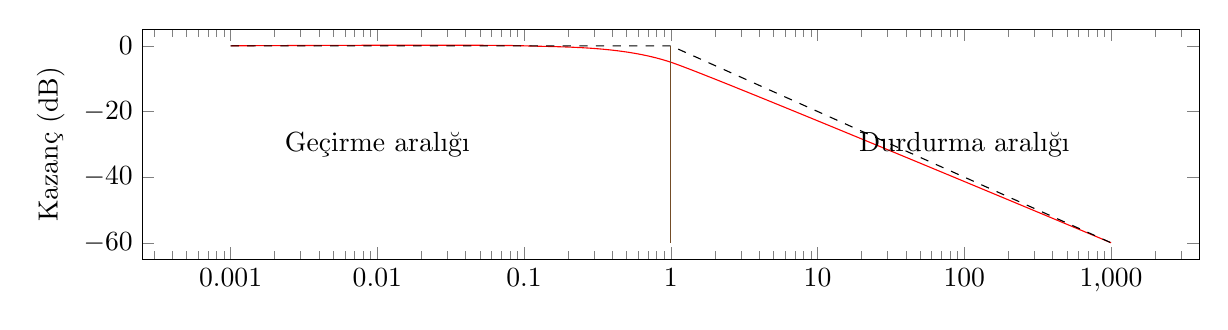
\begin{tikzpicture}
\begin{axis}[
    width=15cm,
	ylabel=Kazanç (dB),
	ymin=-65, ymax=5,
	height=4.5cm,
    xmode=log,
    log ticks with fixed point,
    x filter/.code=\pgfmathparse{#1 + 6.90775527898214}]
\addplot[smooth,red, tension=0.3] table {
		0.000001 0
		0.0001 0
		0.001 -5
		1 -60
	
};
	\addplot[dashed, black] table{
		0.000001 0
		0.001 0
		1 -60	
		};
    \node[] at (axis cs: 0.01,-30) {Geçirme aralığı};
    \node[] at (axis cs: 100,-30) {Durdurma aralığı};

      \addplot +[mark=none] coordinates {(0.001, -60) (0.001, 0)};


\end{axis}
\end{tikzpicture}



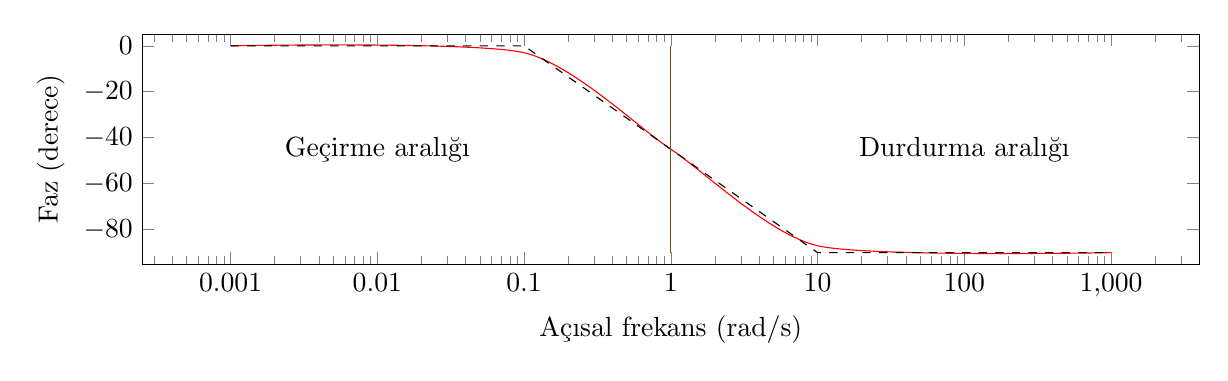
\begin{tikzpicture}
\begin{axis}[
		ylabel=Faz (derece),
		xlabel=Açısal frekans (rad/s),
	ymin=-95, ymax=5,
    width=15cm,
	height=4.5cm,
    xmode=log,
    log ticks with fixed point,
    x filter/.code=\pgfmathparse{#1 + 6.90775527898214}]
\addplot[smooth,red, tension=0.4] table {
0.000001 0
0.0001 -3
0.001 -45
0.01 -87
1 -90
};\label{butter-sinyal};
	\addplot[dashed, black] table{
		0.000001 0
		0.0001 0
		0.01 -90
		1 -90	
		};\label{butter-sinyal-orj};
    \node[] at (axis cs: 0.01,-45) {Geçirme aralığı};
    \node[] at (axis cs: 100,-45) {Durdurma aralığı};
	\addplot +[mark=none] coordinates {(0.001, -90) (0.001, 0)};
\end{axis}
\end{tikzpicture}
\label{butter-stop}
\caption{ Butterworth filtresinden elde edilen sonuç(\ref{butter-sinyal}) ile ideal alçak geçiren filtreden elde edilmiş sonuç(\ref{butter-sinyal-orj}). }
\end{figure}





Derecesi $n$ olan Butterworth filtresinin, frekans düzlemindeki görseller üstünde kullanılması için denklemi,

\begin{equation}
	H(u,v) = \cfrac{1}{1+\left[\cfrac{D(u,v)}{D_0}\right]^{2n}}
	\label{butter-denklem}
\end{equation}

Denklem \ref{butter-denklem}'daki $D_0$, pozitif bir sabittir. Butterworth filtresi, değeri $D_0$'dan küçük her değeri geçirirken, büyük olan değerleri durdurur. Bahsedilen $D_0$, $H(u,v)=1$ ve $H(u,v)=0$ arasında bir geçiş noktasıdır. Sabit bir değer belirtilmesine rağmen; diğer band geçiren filtrelerine kıyasla keskin bir değişim yerine yumuşak ve dalgalanmayan bir değişim sağlamaktadır.

$D(u,v)$, frekans düzleminin orijininden herhangi bir $(u,v)$ noktasına olan Öklid uzaklığını belirtmektedir, yani; $D(u,v)=\sqrt{(u^2+v^2)}$



Bahsedildiği gibi Butterworth filtresinin görsele uygulanabilmesi için görselin, frekans düzlemine taşınması gerekmektedir. Görseli frekans düzlemine geçirmek için \textit{Fast Fourier Transform}una başvurulmuştur. 

Proje kapsamında ilgilenilen sinyallerin frekansları, Butterworth denkleminin yükselen denklem derecesi ile koşum zamanının yavaşlamasından ve 1. derece denklem ile uygun kabul edilebilir sonuçlar gözlemlenmesinden dolayı 1. dereceden Butterworth filtresi kullanılması uygun görülmüştür. Bu karardaki bir diğer faktör de Butterworth filtresinin, belirli bir durdurma aralığı için, denklem derecesi ve gözlemlenen kalıntıların doğru orantılı olmasıdır. Denklem derecesi arttıkça kalıntı şiddeti de artar. Derecesi 1 olan Butterworth filtresinin hiç bir frekansta kalıntı oluşturmayacağı garanti edilir fakat 2 ve daha yüksek dereceler için bu söylenemez. 
\begin{figure}[ht]
    \centering
    \begin{minipage}{0.35\textwidth}
        \centering
	    \includegraphics[width=0.8\textwidth]{butter_placeholder1.jpg} % first figure itself
	    \caption*{a) Gürültülü görsel.}
    \end{minipage}\hspace{1cm}
    \begin{minipage}{0.35\textwidth}
        \centering
        \includegraphics[width=0.8\textwidth]{butter_placeholder2.jpg} % second figure itself
	    \caption*{b) Temizlenmiş görsel.}
    \end{minipage}
	\caption{Gürültüsü yüksek frekanslı ve şiddetli bir görüntünün Butterworth filtresi ile gürültüden arındırılması.}
	\label{butter-ornek}
\end{figure}


\begin{wrapfigure}{r}{0.5\textwidth}
	\vspace{-0.5cm}
	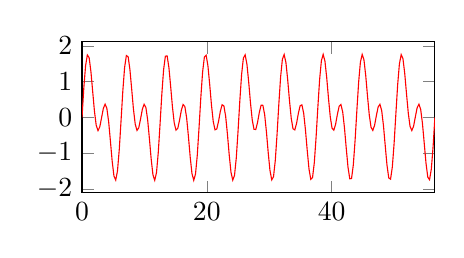
\begin{tikzpicture}
    \begin{axis}[
	    xmin=0,
	    xmax=9*2*pi,
	    height=3.5cm,
	    width=0.5*\textwidth,
     ]
	    \addplot[domain=0:9*2*pi,samples=200,red]{sin(deg(x)) + sin(deg(x*2))};
    \end{axis}
\end{tikzpicture}
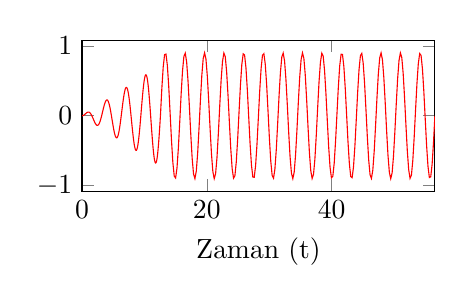
\begin{tikzpicture}
    \begin{axis}[
     xmin=0,
	    xmax=9*2*pi,
	    height=3.5cm,
	    width=0.5*\textwidth,
	    xlabel=Zaman (t),
	    ytick={1,0,-1}
     ]
	    \addplot[domain=0:2*2*pi,samples=200,red]{ ( 1 * deg(x) * sin(deg(x*2))) / 1000 };
	    \addplot[domain=2*2*pi:9*2*pi,samples=200,red]{ (   900 * sin(deg(x*2))) / 1000 };
    \end{axis}
\end{tikzpicture}
	\caption{Yukarıdan aşağıya; İç içe geçmiş 10kHz ve 20kHz sinüs dalgaları ve aynı fonksiyonun 15kHz üstü geçiren Butterworth band filtresinden geçirilmiş hali. }
	\vspace{-0.3cm}
	\label{sekil:butter-graf}
\end{wrapfigure}



Şekil \ref{butter-ornek}'de görüldüğü gibi Butterworth filtresi, şiddeti ve frekansı yüksek gürültülü bir görsel, gerçek gürültüsüz görüntü bilinmese dahi gürültü temizleme konusunda iyi sonuçlar vermekte ve kalıntı oluşturmamaktadır. Görüntü kalitesi, görüntüdeki detayların Fourier transformunda yüksek frekanslı sinüs ve kosinüs dalgalarının, gürültü oluşturan dalgalar ile birlikte durdurulmasından ötürü düşmektedir. Fourier transformunun, belirli bir yakınsama gerektirmesinden ve görüntüdeki sinyalin periyodik olmadığı durumlar olabileceğinden görüntü kalitesinin düşmesi beklenir. 


Butterworth filtresinin alt ve üst kırpma değerlerinin hesaplanabilmesi için Denklem  \ref{butter-denklem}'deki $D_0$ değerinin bilinmesi, bunun için de Nyquist frekansının hesaplanması gerekmektedir. Nyquist frekansı hesaplanırken videonun çekildiği FPS değerinin bilinmesi gerekmektedir. Öngörülen kullanım alanları standart video girişi gerektirdiğinden varsayılan değer 30'dur denilebilir. Belirtilmesi gereken önemli nokta, varsayılan FPS değerinin videonun oynatma sırasındaki FPS'i değil, çekim anındaki FPS'idir.


Nyquist frekansının değeri, normalize ederek yani FPS değerinin yarısını alarak bulunur. Durdurma aralığı için sağladığımız frekansın, Nyquist frekansına bölünmesi gerekmektedir. Butterworth filtresi, sağlanan frekans, fps ve derece bilgileri ile çıktısında, denklemin derecesi $n=1$ olduğundan 2 değer üretir. Bu değerler, sırasıyla pay ve payda polinom katsayılarıdır. Proje kapsamında güçlendirilmek istenen sinyal iki durdurma bölgesinin arasında bulunduğu için iki defa Butterworth filtresinin katsayılarının bulunması gerekmektedir; düşük frekans ve öncesi, yüksek frekans ve sonrası için 2'şer değer bulunması gerekmektedir.  


Şekil \ref{sekil:butter-graf}'te görüldüğü gibi band filtresinden geçirilmiş sinyalin başlangıcı, orijinal sinyal ile genlik olarak örtüşse de şiddet olarak örtüşmemektedir. Bunun nedeni, önceden de belirtildiği gibi Butterworth filtresinin ani değişimler yerine zamanla etkisini göstermesidir. Bu etki, elde edilecek olan videonun başlangıç ve bitişinde gözlemlenebilir. Denklemin $n$ derecesi artarken bu etki, elde edilen denklemlerin eğimi daha fazla olduğundan ötürü azalmakta fakat önceden belirtilen kalıntılardan ötürü istenmeyen sonuçlara neden olmaktadır. 

Butterworth filtresi, oluşturulan ve art arda gelen Laplace piramidi seviyeleri (en düşük ve en düşüğün bir üstündeki seviye) arasında uygulanır. Önceki çalışmamız ve projemizin esas aldığı çalışmaların aksine sadece en alt ve bir üstündeki seviyeler üstünden işlem yaparak işlem zamanından tasarruf edilmiştir. Belirli bir kare ve bu kareden hemen önce gelmiş olan kareler arasında gerekli hesaplamalar yapılır. İki kare arasında Butterworth filtresinin uygulanabilmesi için alçak ve yüksek frekanslar için bulunan 8 değerin ve piramidin kullanılacak olan basamakların ilk karesi referans karesi olarak kullanılması gerekmektedir. 

%				lowpass1 = (-high_b[1] * pyramid[i][0] + high_a[0] * pyramid[i][3] + high_a[0] * pyramid[i][2]) / high_b[0];
%				lowpass2 = (-low_b[1] * pyramid[i][1] + low_a[0] * pyramid[i][3] + low_a[0] * pyramid[i][2]) / low_b[0];
% 			
%				high_a, high_b
%				low_a, low_b

%				\Delta \Phi
%				\delta \phi


\begin{equ}[!ht]
  \begin{equation}
	  \text{filtre1} =  \frac{ [-1 \cdot \Phi [1] \cdot \text{filtre1}] + [\Delta [0] \cdot kare] + [ \Delta [1] \cdot \text{kare}_\text{önceki} ]  }{ \Phi [0] }
	  \label{eq:kod-denklem1}
  \end{equation}


  \begin{equation}
	  \text{filtre2} = \frac{[-1\cdot \phi [1] \cdot \text{filtre2}] + [\delta [0] \cdot \text{kare}] + [\delta [1] \cdot \text{kare}_\text{önceki}]}{\phi [0]}
	  \label{eq:kod-denklem2}
  \end{equation}
\caption*{$\Delta, \delta$; yüksek frekans ile elde edilmiş Butterworth filtresinin pay ve payda bilgileri.}
	\vspace{-0.3cm}
	\caption*{$\Phi, \phi$; alçak frekans ile elde edilmiş Butterworth filtresinin pay ve payda bilgileri.}
\end{equ}


Denklem \ref{eq:kod-denklem1} ve Denklem \ref{eq:kod-denklem2}'de değinilen $\Delta, \delta, \Phi, \phi$ ile ifade edilen değerler, alçak geçiren Butterworth filtresinden elde edilmiş -frekans başına 2- toplam 4 değerdir. Bu değerlerin ardından gelen indis ise bu değerin pay ([0]) veya payda ([1]) olduğunu belirtir. Denklemdeki $filtre1$ ve $filtre2$ değişkenlerinin ilk değerleri, referans olarak filtre uygulanmadan ilk kareye eşitlenir ve her iterasyonun sonunda $\text{kare}_{önceki}$'nin değeri güncel kareye eşitlenir. Böylece her iterasyon, bir önceki filtrelenmiş ve filtrelenmemiş görüntüden etkilenir. Filtre uygulanmış görüntü karesinin değeri $filtre1 - filtre2$ ile bulunur ve çıkışa, güncel kare ile toplanarak aktarılabilir.

Değinildiği gibi görüntü karelerinin arasındaki değişimler, her iterasyonda $highpass$ ve $lowpass$ değerleri bir önceki görüntü karesinin değerlerini içermesi sayesinde hesaplanır. 

\subsection{Filtrelenmiş Laplace Piramitlerinden Video Elde Etme}{\label{gauss-piramit-video}}

Bölüm \ref{gauss-piramit}'de elde edilen piramidin seviye sayısı, kullanıcının isteğine göre değişkenlik göstereceğinden orijinal video boyutunun saklanması gerekmektedir. Bölüm \ref{butterworth-filtre}'de elde edilen filtre uygulanmış piramit seviyelerinin en üstteki basamağının, bahsedilen bu orijinal video boyutuna çıkarılması gerekmektedir. Bunun için, görüntü istenen boyuta çıkana kadar Denklem \ref{expand-denklem} tekrarlanır. Gauss piramidinin en üst basamağının -boyut olarak en küçük basamak- çözünürlüğü düşük olduğundan ve bu piramit basamağı orijinal boyuta yükseltileceğinden gözlemlenen değişimlerin hassaslığı düşmektedir. Bu durum istenmeyen sonuçlara neden olmamakta, aksine görüntüdeki ani değişimleri ve gürültüyü yüksek oranda azaltmaktadır. 


İşlemler sonrasında elde edilen görüntü sekansı, orijinal videoda değişkenlik göstermeyen kısımları içermez. 



\subsection{Video ile Laplace Piramitlerinin Birleştirilmesi}{\label{sec:birlestirme}}

Bölüm \ref{gauss-piramit-video}'te elde edilen \textit{maske}, orijinal videodaki değişimler kadar zayıftır ve bir katsayı ile çarpılmadan orijinal video ile birleştirilirse hiç bir değişim gözlemlenemez (Bölüm \ref{birinci-dereceden}, Taylor serisi ile yaklaşılan değer). Bu değişimlerin gözlemlenebilmesi için kullanıcıdan alınan bir katsayı ile çarpılıp orijinal video ile toplanması gerekmektedir. Bu adımdaki katsayı, Bölüm \ref{birinci-dereceden}'de değinilen $\alpha$ sabitidir, Elde edilen görüntü sekansı, proje kapsamında elde edilmek istenen değişimlerin abartılmış şekilde görülebildiği videodur. Şekil \ref{sonuc-ort}'te orijinal sinyal ile artırılmış sinyal gözlemlenmektedir.


% (?) axis adlarını düzelt
\begin{figure}[h]
\centering
\begin{tikzpicture}
\begin{axis}[
	width=0.9 * \textwidth,
    	height= 4.5cm,
	xlabel=Milisaniye (ms),
	ylabel=Parlaklık (0-255),
	yticklabels={80,100,120,140,160,180}
    ]

\addplot +[mark=none, red]
	table  {maske_amp1.txt};\label{arttirilmis-sinyal}
	\addplot +[mark=none, blue]
	table {orjinal1.txt};\label{orijinal-sinyal}
\end{axis}
\end{tikzpicture}
	\caption{Görüntü karelerinin parlaklık ortalaması. Orijinal sinyal(\ref{orijinal-sinyal}) ve nabız bilgisi arttırılmış sinyal(\ref{arttirilmis-sinyal}). } 
\label{sonuc-ort}
\end{figure}

\vspace{-1cm}

\subsection{Hızlı Fourier Dönüşümü}



\ref{sec:birlestirme}'de nabız bilgisini arttırıp orijinal video ile birleştirdikten sonra kullanıcıya görsel bir sonuç sunduk. Nabız bilgisinin sayısal olarak kullanıcıya aktarılabilmesi için elde edilen bu videoya Fourier dönüşümünün uygulanması ve sinyal içerisinde bulunan nabız bilgisinin izole edilmesi gerekmektedir. Sinyalden nabız algılama konusunda kullanılan diğer yöntemlerin yerine Fourier dönüşümünün kullanılmasının sebebi uygulama kolaylığı ve işlem zamanından tasarruftur. Projeye fazladan kütüphane eklememek ve kurulum aşamasında karmaşıklık oluşturmamak adına Cooley-Tukey FFT algoritması implemente edilmiştir. 

Bellek kullanımı açısından naif bir yöntem olsa da video girişi ve ilgilenilen zaman aralığı, $10\text{saniye}\cdot30\text{FPS}=300$ kare olduğu öngörüldüğünden performans darboğazı yaratmamaktadır. Algoritma implementasyonu rekürsiftir, "parçala ve fethet" prensibi ile çalışır. Fourier dönüşümü alınacak olan $x$ dizisi, indisi tek ve çift olan dizilere ayrılır ve fonksiyon bu değerler ile tekrar çağrılır. Çağrılan her alt fonksiyonun orijinal $x$ dizisinden elde edilmiş alt dizinlere erişim hakkı olduğundan fonksiyonun çıktısı yine $x$ dizisine aktarılır ve bütün alt fonksiyonların koşumu bittiğinde sonlanmış sayılır. Diziyi tek ve çift indislere böldüğünden giriş dizisinin ikinin katı boyutunda olması gerekmektedir. Proje kapsamında 30 FPS, 10 saniye olan bir video girişinden sonuç elde edilmeye çalışıldığından bu değere en yakın ikinin katı olan 256, $x$ dizisinin boyutu olarak önceden seçilmiştir. Bu durum 256 kareden kısa videolarda programın hata ile sonlanacağını belirtir. Proje kapsamında kullanılmayacağından ters Fourier dönüşümü implemente edilmemiştir. 

\begin{figure}[h]
\centering
\begin{tikzpicture}
\begin{axis}[
	width=0.9 * \textwidth,
    	height= 4.5cm,
	xlabel=Frekans bölmesi,
	ylabel=Gücün karesi
    ]

\addplot+[thin,red,mark options={scale=0.7}]
table  {fourier1.txt};
\end{axis}
\end{tikzpicture}
\caption{Örnek videodan elde edilmiş sonuç üzerine uygulanmış FFT'nin sonucu. FFT'nin sonucu simetrik olduğundan görsele 256 örnekten 128 tanesi dahil edilmiştir. } 
\label{ftt-sonuc}
\end{figure}


FFT'nin sonucunda, $N$ örnek kadar frekans bölmesi elde edilir. Sonsuz uzayda yapılan işlemlerin aksine, gerçek dünyada Fourier dönüşümünden elde edilen bilginin çözünürlüğü örnekleme sayısı ve frekansa bağlıdır. Bu nedenden ötürü 30 FPS, 10 saniye bir video girişinden her bir frekans bölgesinin $0.1 \; Hz$ frekans aralığına düştüğünü görmekteyiz. Örnek olarak; 30 FPS, 10 saniye bir video girişinden bireyin nabzının 10. frekans bölmesinde artış yarattığını gözlemlersek bireyin nabzının 0.95 $Hz$ ile 1.05 $Hz$ arasında olduğunu söylemekteyiz. Verilen örnek için çözünürlük, dakikada $\pm$ 3 nabızdır. Spesifik olarak $n.$ frekans bölmesinin ifade ettiği frekans aralığını bulmak için;

\begin{equation}
\label{eqn:fft}
\text{n. bölmenin frekansı} = n * \frac{\textrm{örnekleme frekansı}}{\text{örnekleme sayısı}}
\end{equation}
denkleminden yararlanılır. Görüleceği üzere 0'dan örnekleme frekansına kadar olan bütün frekansların bölmelerini elde etmiş olmaktayız. Şekil \ref{ftt-sonuc}'de de gözlemlendiği gibi her video girişi için bir frekans bölmesinde yoğunlaşma gözlemlenmemektedir. Gerçek dünyada DFT uygulamalarında \textit{sızıntı} durumu ile karşılaşılmaktadır, bu durum uygulamamızda nadir olarak gözlemlense de öncesinde bahsedilen durum sık sık karşımıza çıkmaktadır. Bu sorunu çözmek için girilen frekans aralığında gözlemlenen en güçlü 3 frekans bölmesinin ortalamasında bulunan frekans bölmesi sonuç olarak alınmak istenmiş fakat bu yaklaşım da her zaman doğru sonuçlar üretmemektedir. Buna rağmen; hiç bir çıktıda seçilen frekans bölgesinin iki ucunda birbirleri ile çelişen iki tepe değer saptanmamış ve her zaman güçlü bir frekans bölmesinin etrafında bir veya daha fazla göreli olarak güçlü frekans bölmesi gözlemlenmiştir.  



\subsection{Optimizasyon}

Önceki bölümlerde, geçmiş çalışmalara göre performans artışı sağladığımızdan bahsetmiştik. Bu performans iyileştirmelerini iki ana başlıkta inceleyebiliriz; RGB görüntü karelerinin ayrıştırılması ve video girişinin belleğe alınmadan işlemlerin gerçekleştirilmesi. 

Kullanıcı arayüzünde, kullanıcıya RGB kanallarının sadece bir tanesi üzerinde işlem yapılabilmesi seçeneğini sunduk. Bu seçenek sayesinde işlem yapılacak olan görüntü sekansının boyutunu $\sfrac{1}{3}$ oranında azalttık. Bu seçenek kullanılacak ise özellikle kırmızı ve yeşil kanalların kullanılması önerilir. Tasarım aşamasında kırmızı, yeşil ve mavi kanallarının ortalamasını alarak işlem yapılması düşünülmüş fakat nabız değişimi, örnek verecek olursak kırmızı kanalda artışa sebepiyet verirken yeşil kanalda düşüşe neden olmaktadır. Bu nedenden ötürü görüntünün ortalaması alınırsa nabız sinyali algılaması zorlaşmaktadır. Anlaşılacağı üzere bu iyileştirme kullanıldığında kullanıcıya sunulacak olan görsel çıkış siyah beyaz olacaktır.

İkinci iyileştirme ise görüntü sekansının belleğe alınmadan işlem yapılmasıdır. Önceki tasarımlarda, örnek verecek olursak 30 FPS, 10 saniye ve 720P çözünürlüğündeki videoların -sıkıştırma algoritması farketmeksizin- belleğe alınması için $30\cdot10\cdot1280\cdot720\cdot3=829440000\; byte$ yani $0.85\;GB$ ayrılması gerekmektedir. Piramit basamaklarının oluşturulması ve program çıktısının saklanması, en az video girişinin iki katı kadar bellek kullanmaktadır.Ek olarak, bütün video girişinin belleğe alınarak işlem yapılması gerçek zamanlı görüntü işlemesini imkansız kılmaktadır. 


Videonun belleğe alınmadan üstünde işlem yapılabilmesi için okunan her karenin Laplace piramidinin oluşturulması gerekmektedir. Piramidin en alt 2 basamağı kullanılacağından diğer seviyeler işlem anında bellekten silinmektedir. Denklem \ref{eq:kod-denklem}'da değinildiği gibi Butterworth filtresinin, önceki görüntü karesi ve bu görüntü karesine Butterworth filtresi uygulanmış halinin saklanması gerekmektedir. Uyguladığımız performans iyileştirmesi yöntemi ile; önceki görüntü karesi, bu karenin filtrelenmiş hali, güncel kare, bu karenin filtrelenmiş hali ve güncel karenin iki adet piramit basamağı saklanması gerekmektedir. Önceki örnek için sadece video girişinden elde edilen bilgiler için $0.85\cdot3=2.55\; GB$ yer ayrılırken optimizasyon sonucu programın \textit{toplamda} kullandığı bellek miktarı $100\;MB$'a düşmüştür. 


\subsection{Kullanıcı Arayüzü}

Kullanıcı arayüzü Şekil \ref{fig:arayuz}'de görüleceği üzere programın giriş/çıkış, performans iyileştirmesi ve temel ayarlar olarak ayrılmıştır. Giriş/Çıkış kısmında kamera girişi ve geliştirdiğimiz hareketin azaltılması seçeneği yer almaktadır. Giriş kamera olarak seçildiğinde dosya yolu devre dışı bırakılır ve bilgisayara bağlı ilk kamera kullanılır. Performans kısmında ise yapılan performans iyileştirmelerine rağmen gerçek zamanlı işlem yapamayacak donanımdaki bilgisayarlar gözetilerek eklediğimiz RGB seçenekleri mevcuttur. Bu seçeneklerden biri seçildiğinde diğerleri devre dışı bırakılır ve tüm işlemler sadece belirtilen kanal üzerinden gerçekleştirilir. Ortam koşullarına göre değişkenlik gösterse de kullanıcıya, bu performans iyileştirmesi kullanılacaksa öncelikle yeşil kanalın denenmesi önerilir. Temel ayarlarda ise önceki bölümlerde değinilen alçak ve yüksek frekans, alfa ve piramit seviye parametreleri yer almaktadır. Bu değerlrin tamamı tek bir yazı dosyasına, projenin çekirdek kodunun okunması üzere kaydedilir.

\begin{figure}[h]
	\centering
	\includegraphics[width=9cm]{arayuz.jpg}
	\caption{Kullanıcıdan parametrelerin alındığı arayüz.}
	\label{fig:arayuz}
\end{figure}


Kullanıcı arayüzü ve projenin çekirdek kodu ayrı programlar olduklarından aralarındaki iletişim dosyalara yazma işlemi ile gerçekleştirilmiştir. Kullanıcı arayüzü, ayarların tamamı \textit{config.txt} dosyasına yazar, çekirdek kod ise bu dosyadan ayarları her saniyenin üçte biri süresinde tekrar okur. Kamera, Laplace, RGB ve dosya yolu haricindeki seçenekler program koşum sırasında değiştirilebilmektedir. Böylelikle kullanıcı ortam koşulları için doğru olan ayarları bulmak için kamera veya video akışını durdurmak zorunda bırakılmamıştır. Çekirdek kod, Fourier dönüşümünden sonra bulunan nabız bilgisini \textit{stdout}'a yazar ve C\# yazılan bu bilgiyi okuyarak "Nabız Sonucu" bölmesindeki değerleri günceller. 


\newpage
\section{KISITLAR}\label{sec:kisitlar}

Giriş videosunun çözünürlüğü arttıkça çıkış görüntüsününü hesaplanması, videonun boyutları ile doğru ve üssel bağıntılıdır. Fakat seçilen görüntü piramidinin derinliği ile işlem zamanının arasında lineer veya üssel bir ilişki yoktur. Bunun nedeni; görüntü piramidi seviyesi arttıkça harcanan bellek miktarı artsa da uygulanacak filtrelerin, azalan görüntü uzayındaki hesaplama hızı düştüğünden işlem genel olarak hızlanır.

Görüntü piramidinin yeteri kadar derin seçilmemesi durumunda görüntüdeki ilgilenilmeyen bölgelerdeki değişimin de gösterilmesine neden olur. Yüz bölgesinde değişkenlik arandığından 400x400 büyüklüğündeki bir görüntü için ideal piramit derinliği 3 ile 5 değerleri arasındadır. Bu değerler sırası ile; daha keskin veya daha yumuşak geçişler gözlemlenir. Önceki çalışmamıza göre piramit seviyelerindeki artış program çıktısında olumsuz sonuçlara neden olmamaktadır.

Bahsedilen işlem zamanının optimum olması için giriş videosunun çözünürlüğünün olabildiğince küçük, piramit seviyesi seçiminin ise olabildiğince büyük olması gerekmektedir. Yüksek çözünürlüklü girişler işlem zamanını arttıracağından, gereğinden fazla seviyeli piramitler ise uygulanacak olan maskenin çözünürlüğünü düşürüceğinden tercih edilmez.

Nabız bilgisi okunacak olan bireyin bulunduğu ortam, programa sağlanan parametrelerden daha önemlidir. Işık bakımından gürültülü, bireyin düzenli olarak hareket etmesi sonucu, parametrelerin oluşturucağı değişiklikten daha fazla etkliler.


\newpage

\section{SONUÇ VE ÖNERİLER}{\label{sonuclar}}

Projemizin kaynak kodları, test görüntüleri ve kurulum için gerekli dosyalar ilgili link ve atıftadır.\cite{kod_bizim} 

Önceki tasarımımız ve protitipimize kıyasla gürültüsüz ve gerçek zamanlı çalışan bir uygulama geliştirdik. Orijinal çalışmada geliştirilen uygulama aynı video girişini 6 dakikada, prototipimiz 30 saniyede, bu tezde değinilen çalışma ise gerçek zamanlı işlemektedir. Orijinal çalışmada, kullanıcı için sayısal bir sonuç üretilmemiş olup sadece nabzın arttırıldığı görüntü sonucu sağlanmıştır. Çalışmamızda kullanıcını için kullanım kolaylığı sağlanmış ve sayısal bir sonuç üretilmiştir. 

Önceki bölümlerde de değinildiği gibi filtreleme yöntemi için farklı filtreler kullanılabilir fakat bu çalışmanın özelleşmiş donanım ile tasarımı açısından Butterworth filtresi, implemente edilmesi kolay olduğundan bundan sonraki çalışmalar için -sonucu önemli ölçüde etkilemeyecekse- filtrenin değiştirilmemesi -kişisel görüşümüz olarak- tavsiye edilir. 

Filtrelemeden geçirilmiş görüntünün, orijinal video ile birleştirilme aşamasında $\alpha$ sabiti ile çarpılmadan önce karesinin alınması, çıkıştaki gürültüyü azaltabilmektedir. Bu yaklaşım özellikle eski model, gürültülü görsel sağlayan kameralar için uygulanabilir fakat kameraların ürettiği gürültü öngörülemeyeceği için bu çözüm genellenemez.

Önceki bölümlerde de değinildiği gibi nabız bilgisi edinmek istenilen bireyin iyi ışıklandırılmış ortamda bulunması ve kameranın mümkün olduğunca sabit tutulmuş olması gerekmektedir. İzole edilmek istenen frekans aralığının aşırı dar olmaması, dar olması durumunda ise $\alpha$'nın frekans darlığına göre arttırılmış olması gerekmektedir.

Video giriş aygıtının çekim sırasında dinamik ISO değerleri yerine çekim öncesinde ortam koşullarına uygun ISO değerlerinin seçilmesi tavsiye edilir. Bu tavsiyenin gerekçesi; test edilen çoğu kameranın çekim anından önce değil, çekim sırasında ISO değerlerinin düzenlemesinden kaynaklıdır. Bu durum gereğinden uzun süre boyunca örnek alınmasını gerektirir.

\newpage


\addcontentsline{toc}{section}{KAYNAKLAR}
\bibliography{ref.bib}
\bibliographystyle{ieeetr}


\newpage 

\section*{STANDARTLAR VE KISITLAR FORMU}

Projenin hazırlanmasında uyulan standart ve kısıtlarla ilgili olarak, aşağıdaki soruları cevaplayınız.

\begin{enumerate}
	\item Projenizin tasarım boyutu nedir? (Yeni bir proje midir? Var olan bir projenin tekrarı mıdır? Bir projenin parçası mıdır? Sizin tasarımınız proje toplamının yüzde olarak ne kadarını oluşturmaktadır?)

\vspace{0.3cm}
\noindent\fbox{		\parbox{\textwidth}{
	Orijinal tezde matematiksel ispatı yapılmış fakat takip edilmesi gereken işlem adımlarına değinilmemişti. Performans iyileştirmeleri ve algoritma adımlarında değişikliğe gidildiğinden, kullanıcıya arayüz sağlandığından ve hareketi azaltmak üzere Laplace piramitlerinin kullanılmasından ötürü \%70'sini bizim tasarımımız oluşturmaktadır. }}

\vspace{0.3cm}
	\item Projenizde bir mühendislik problemini kendiniz formüle edip, çözdünüz mü? Açıklayınız.
\vspace{0.3cm}
\noindent\fbox{		\parbox{\textwidth}{
	Matematiksel ispattan gerçek dünyadaki gerçeklenmesine geçme adımında birden fazla problemle karşılaştık. Belli frekans aralığını durdurma işlemi için filtre seçimi ve görüntü piramitlerinin oluşturulması adımlarının gerçeklenmesi problemlerini çözdük.}}
\vspace{0.3cm}
	\item Önceki derslerde edindiğiniz hangi bilgi ve becerileri  kullandınız?
\vspace{0.3cm}
\noindent\fbox{		\parbox{\textwidth}{
	Sinyaller ve Sistemler dersinden sinyal işleme, Görüntü İşleme dersinden Gauss piramitlerinin oluşturulması ve Mühendislik Matematiği dersinden Fourier dönüşümü hakkında öğrendiklerimizi kullandık. }}
\vspace{0.3cm}
	\item Kullandığınız veya dikkate aldığınız mühendislik standartları nelerdir? (Proje konunuzla ilgili olarak kullandığınız ve kullanılması gereken standartları burada kod ve isimleri ile sıralayınız).
\vspace{0.3cm}
\noindent\fbox{		\parbox{\textwidth}{
	OpenCV (görüntü piramitlerinin oluşturulması), sinyal filtreleri (Butterworth, FIR), Cooley-Tukey Fourier algoritması (sinyalden nabız bilgisinin elde edilmesi) ve C\# arayüz kütüphanelerinden yararlandık.	 }}
\

	\item Kullandığınız veya dikkate aldığınız gerçekçi kısıtlar nelerdir? Lütfen boşlukları uygun yanıtlarla doldurunuz.
		\begin{enumerate}
			\item Ekonomi
\vspace{0.3cm}
\noindent\fbox{		\parbox{0.93\textwidth}{
			Projenin ölçeklenme fırsatına sahip olması için işlem zamanından ve bellek kullanımından tasarruf edilmeye çalışılmıştır.}}
\vspace{0.3cm}
			\item Çevre sorunları
\vspace{0.3cm}
\noindent\fbox{		\parbox{0.93\textwidth}{
				Proje herhangi bir çevre sorunu teşkil etmemektedir.}}
\vspace{0.3cm}
			\item Sürdürlebilirlik
\vspace{0.3cm}
\noindent\fbox{		\parbox{0.93\textwidth}{
				Proje sürdürülebilirlik açısından herhangi bir sorun teşkil etmemektedir.}}
\vspace{0.3cm}
			\item Üretilebilirlik
\vspace{0.3cm}
\noindent\fbox{		\parbox{0.93\textwidth}{
				Projenin program kısmında tekrarlanabilirliğinin kolay olması adına sektörde kabul görmüş kütüphaneler kullanılmıştır.}}
\vspace{0.3cm}
			\item Etik
\vspace{0.3cm}
\noindent\fbox{		\parbox{0.93\textwidth}{
				Proje, bireyin rızası olmadan nabzını ölçmekte kullanılabilir. Bu durum etik açısından sorun teşkil etmektedir. }}
\vspace{0.3cm}
			\item Sağlık
\vspace{0.3cm}
\noindent\fbox{		\parbox{0.93\textwidth}{
				Projenin sağlık açısından herhangi kısıtı yoktur.}}
\vspace{0.3cm}
			\item Güvenlik
\vspace{0.3cm}
\noindent\fbox{		\parbox{0.93\textwidth}{
				Proje güvenlik açısından bir sorun teşkil etmemektedir.}}
\vspace{0.3cm}
			\item Sosyal ve politik sorunlar
\vspace{0.3cm}
\noindent\fbox{		\parbox{0.93\textwidth}{
				Proje etik kısmında bahsedilen kısıtlar haricinde bir sosyal ve politik sorun içermemektedir.}}
\vspace{0.3cm}
		\end{enumerate}

\end{enumerate}

\end{document}
